\section{Methods}
The first study involved a systematic literature review to identify randomized controlled trials (RCTs) that investigated the effects of health wearable-based physical activity interventions of individuals with overweight/obesity and chronic comorbidities. This was followed by a statistical analysis of multiple treatments. This analyzed direct and indirect comparisons of interventions, and helped synthesize the effectiveness of each intervention strategy compared to other control conditions. Fig. \ref{fig:PRISMA-01} shows the PRISMA\footnote{\label{foot:PRISMA}PRISMA (Preferred Reporting Items for Systematic Reviews and Meta-Analyses) is an evidence-based minimum set of items for reporting in systematic reviews and meta-analyses \cite{ref06}} diagram for the literature search process flow.
\begin{figure}[H]
     \centering
     \begin{subfigure}[b]{0.52\textwidth}
         \centering
         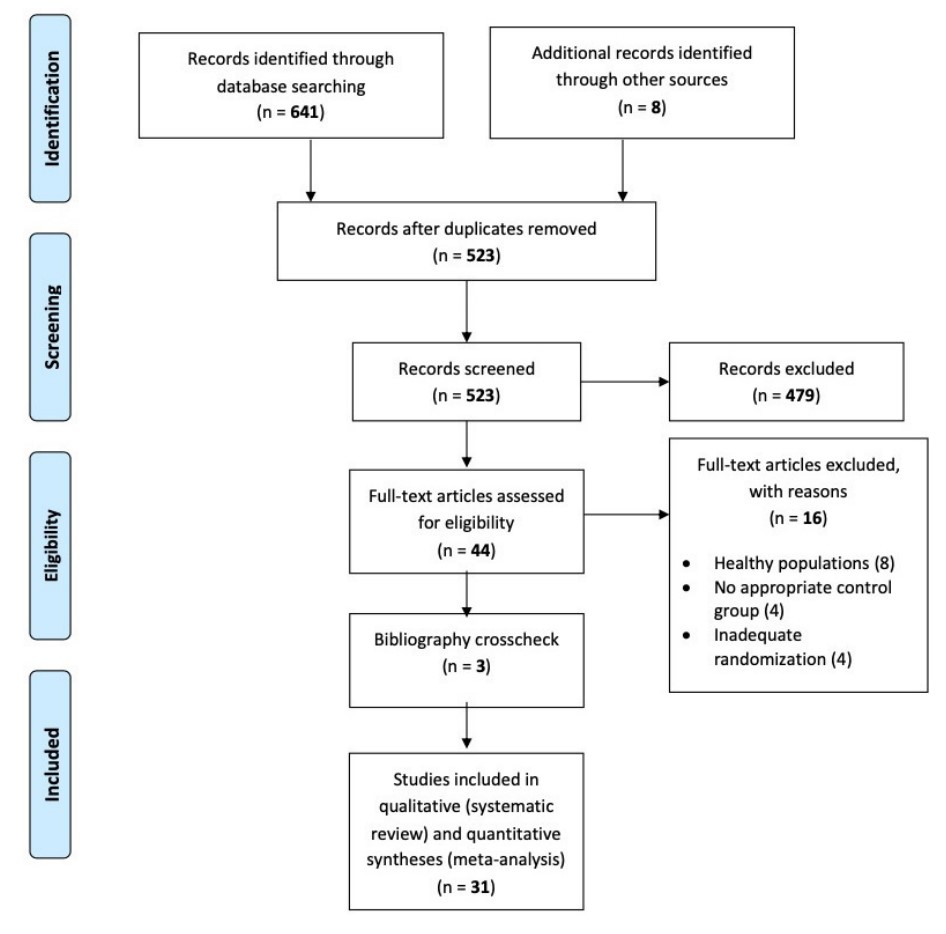
\includegraphics[width=\textwidth]{assets/LittProcessFlow-Case01.jpg}
         \caption{PRISMA flow chart for systematic reviews \cite{ref01}}
         \label{fig:PRISMA-01}
     \end{subfigure}
     \hfill
     \begin{subfigure}[b]{0.46\textwidth}
         \centering
         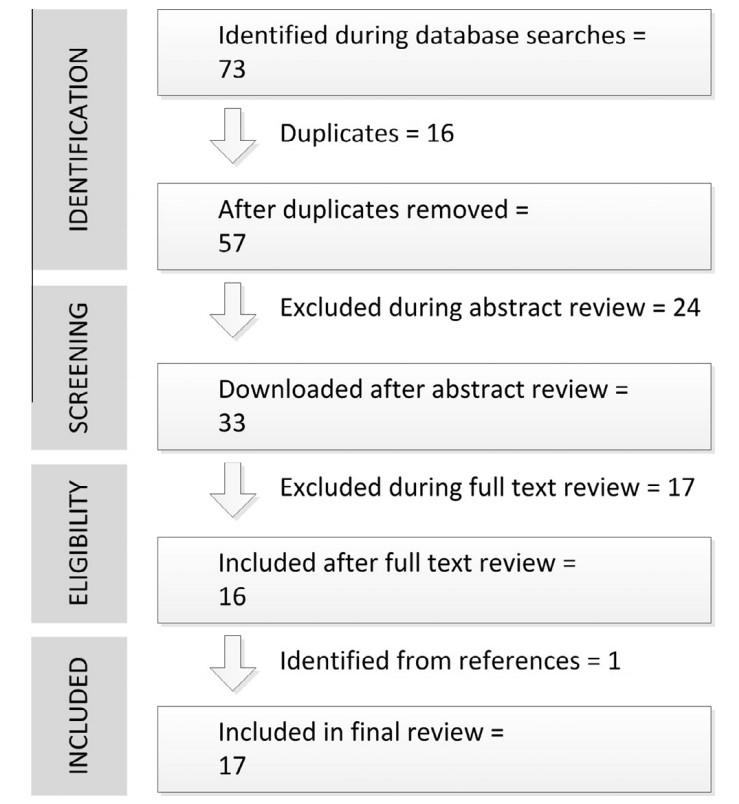
\includegraphics[width=\textwidth]{assets/LittProcessFlow-Case03.jpg}
         \caption{Process flow for literature search \cite{ref03}}
         \label{fig:PRISMA-03}
     \end{subfigure}
\end{figure}
The second study conducted a clinical trial where 471 adult participants were enrolled between October 2010 and October 2012, and data collection was completed by December 2014. Participants were initially placed on a low-calorie diet, prescribed increases in physical activity, and had group counseling sessions. After 6 months, the interventions added telephone counseling sessions, text message prompts, and access to study materials on a website. At this point, participants randomized to the standard intervention group initiated self-monitoring of diet and physical activity using a website while those randomized to the enhanced intervention group were provided with a wearable device and accompanying web interface to monitor diet and physical activity. The flow of participants throughout the study is depicted in Fig. \ref{fig:ParticipantFlow}.

The third study involved a review of 17 clinical studies between 2014 and 2016, with the exception of one published in 2011. Participant demographics, device features, watch applications and methods, and technical challenges were abstracted from included studies. Most studies employed the use of consumer-grade smart watches and enrolled participants with few exclusion criteria to validate smart watch function. The studies focused on activity monitoring, heart rate monitoring, diabetes self-management, and detection of non-ideal medical behaviors. Fig. \ref{fig:PRISMA-03} represents the PRISMA flowchart followed by the authors in selecting and studying previous literature.
\begin{figure}[!htb]
    \centering
    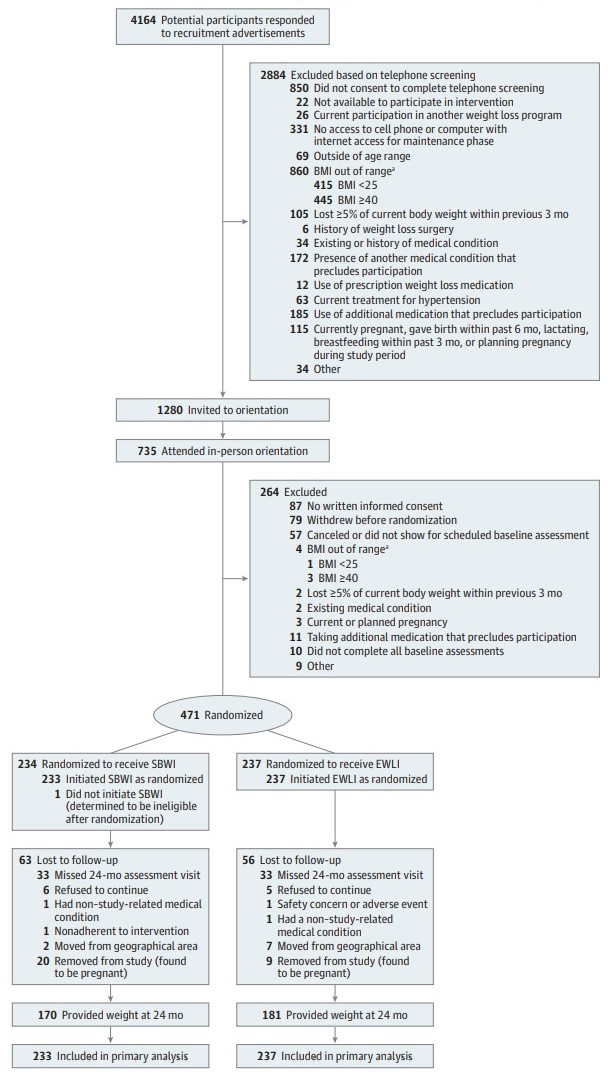
\includegraphics[width=0.7\textwidth]{assets/ParticipantFlow-Case02.jpg}
    \caption{Flow of Participants in the IDEA Study \cite{ref02}}
    \label{fig:ParticipantFlow}
\end{figure}
